\documentclass[11pt,a4paper]{article}

% 1. Llamada al archivo de librerías y configuraciones
% --- Codificación e Idioma ---
\usepackage[utf8]{inputenc}
\usepackage[spanish, es-tabla]{babel} % Idioma español y uso de "Tabla" en lugar de "Cuadro"

% --- Matemáticas y Física ---
\usepackage{amsmath, amssymb, amsfonts} % Símbolos y entornos matemáticos
\usepackage{siunitx} % Excelente para escribir unidades con formato profesional (ej. \SI{220}{\ohm})

% --- Gráficos y Tablas ---
\usepackage{circuitikz} % Para dibujar circuitos eléctricos
\usepackage{subcaption} % Para subfiguras dentro de una figura
\usepackage{graphicx} % Para insertar imágenes
\usepackage{float} % Para forzar la posición de imágenes y tablas con [H]
\usepackage{booktabs} % Para tablas con líneas profesionales (\toprule, \midrule, \bottomrule)
\usepackage{csvsimple} % Para importar datos directamente desde archivos CSV
\usepackage{pgfplots} % Para generar gráficos a partir de datos
\usepackage{multicol} % Para crear columnas en tablas o texto
\pgfplotsset{compat=1.18} % Versión de compatibilidad para pgfplots

% --- Formato y Diseño ---
\usepackage{geometry} % Configuración de márgenes
\geometry{
    a4paper,
    top=2.5cm,
    bottom=2.5cm,
    left=2.5cm,
    right=2.5cm
}
\usepackage{fancyhdr} % Para personalizar encabezados y pies de página
\usepackage{hyperref} % Para que el índice y las referencias sean enlaces clickeables
\hypersetup{
    colorlinks=true,
    linkcolor=black,
    filecolor=magenta,
    urlcolor=blue,
    citecolor=black
}
\usepackage[bottom, hang, flushmargin]{footmisc} % Para mejorar la apariencia de las notas al pie



\begin{document}

% 2. Llamada a la carátula
\begin{titlepage}
    \centering

    % LOGO
    % 
\includegraphics[width=0.45\textwidth]{ITBA.PNG}\par % Descomentar si tienes la imagen
    \vspace{3cm}

    % UNIVERSIDAD
    {\scshape\LARGE Instituto Tecnológico de Buenos Aires \par}
    \vspace{2cm}

    % TÍTULO
    {\Huge\bfseries Trabajo Práctico N°1 \par}
    \vspace{0.5cm}
    {\Large Curvas Caracteristicas \par}
    \vspace{0.5cm}
    {\large Física III \par}

    \vspace{4cm}

    % GRUPO E INTEGRANTES
    \begin{flushleft}
    {\Large\textbf{Grupo: 2}\par}
    \vspace{0.5cm}

    {\Large\textbf{Integrantes:}\par}
    \vspace{0.3cm}
    \begin{tabular}{l r}
        CÁCERES SMOLER, MARIANO      & 66858 \\
        CASTRO, TOMÁS                & 66905 \\
        ROSA FERNANDEZ, ENZO NICOLÁS & 66518 \\
        MARRESE, MÁXIMO              & 66223 \\
    \end{tabular}
    \end{flushleft}

    \vfill

    % FECHAS
    \begin{flushleft}
    {\large \textbf{Fecha de realización:} 17/04/2026\par}
    {\large \textbf{Fecha de entrega:} 24/04/2026\par}
    \end{flushleft}

    \vspace{0.6cm}

    % SECTOR DE EVALUACIÓN PARA EL DOCENTE
    \begin{flushleft}
    {\large\textbf{Observaciones del docente:}}\par
    \vspace{0.2cm}
    \framebox[\linewidth]{\rule{0pt}{3cm}}

    \vspace{0.8cm}

    \begin{tabular}{@{}p{0.45\linewidth} p{0.45\linewidth}@{}}
        \textbf{Fecha de aprobación:} \hrulefill & \textbf{Firma:} \hrulefill \\
    \end{tabular}
    \end{flushleft}

    \vspace{0.5cm}
\end{titlepage}


% Índice de contenidos
\newpage
\tableofcontents
\newpage

% 3. Llamada a la sección de objetivos y resúmen
\section{Objetivos}
El objetivo principal de esta práctica de laboratorio es relevar y determinar las curvas características intensidad-tensión ($I$ vs $V$) para distintos componentes eléctricos de dos terminales, con el fin de analizar su linealidad.

Los elementos específicos a evaluar son:
\begin{itemize}
    \item Resistencia de carbón depositado.
    \item Lámpara de filamento de tungsteno.
    \item Diodo semiconductor de silicio.
    \item Diodo emisor de luz (LED).
\end{itemize}

\vspace{0.5cm}

\section{Resumen}
Para comprender la naturaleza de la conducción eléctrica en distintos dispositivos, resulta fundamental caracterizar empíricamente la relación entre la diferencia de potencial aplicada a un componente y la corriente que lo atraviesa. Esta experiencia tuvo como propósito contrastar el comportamiento de elementos óhmicos (lineales) frente a elementos no óhmicos (no lineales), identificando empíricamente las desviaciones de la Ley de Ohm provocadas por efectos térmicos o por la naturaleza de los materiales semiconductores.

Para llevar a cabo este análisis, se implementó un circuito de medición compuesto por una fuente de tensión continua variable, un amperímetro dispuesto en serie, un voltímetro en paralelo y el elemento bajo ensayo. Aumentando progresivamente la tensión suministrada — y asegurando no exceder los valores máximos de tensión y corriente admitidos por cada componente — se relevaron los distintos pares de valores de corriente y tensión. Finalmente, con los datos obtenidos, se construyeron las gráficas correspondientes a las curvas características $I=f(V)$ de cada elemento, permitiendo así evaluar visual y analíticamente su comportamiento y linealidad.

\vspace{0.8cm}


\pagebreak
% 4. Llamada a la sección de introducción teórica
\section{Introducción Teórica}

\subsection{Curvas Características e Idealidad}
La relación entre la corriente eléctrica $I$ que atraviesa un componente y la diferencia de potencial $V$ aplicada entre sus terminales se denomina \textbf{curva característica}.

Dependiendo de esta relación, clasificamos los elementos en:
\begin{itemize}
    \item \textbf{Elementos Óhmicos (Lineales):} Son aquellos donde la corriente es directamente proporcional a la tensión ($V = I \cdot R$). Su gráfica es una recta que pasa por el origen, y su resistencia $R$ permanece constante independientemente del valor de $V$ o $I$.
    \item \textbf{Elementos No Óhmicos (No Lineales):} Son aquellos donde la relación no es lineal. En estos casos, la resistencia puede variar según el punto de operación debido a factores como la temperatura o la estructura interna del material (como en los semiconductores).
\end{itemize}

\vspace{0.5cm}

\subsection{Resistores de Carbón Depositado}
Constituyen el ejemplo típico de componente lineal fijo. Estos dispositivos están compuestos por una varilla cerámica sobre la cual se deposita una fina capa de carbón.
\begin{itemize}
    \item \textbf{Composición:} Carbón pirolítico sobre soporte cerámico.
    \item \textbf{Parámetros técnicos:} Para la práctica de laboratorio, se definen por su \textbf{resistencia nominal} (el valor óhmico esperado por el fabricante) y su \textbf{tolerancia} (el margen de error expresado en porcentaje dentro del cual se halla el valor real).
    \item \textbf{Comportamiento:} Presentan una oposición al paso de la corriente constante dentro de sus límites nominales de potencia, siguiendo estrictamente la Ley de Ohm.
\end{itemize}

\vspace{\fill}

\pagebreak

\subsection{Lámpara de Filamento de Tungsteno}
Es un dispositivo no lineal debido a fuertes efectos térmicos. Consiste en un filamento de tungsteno encerrado en una ampolla con gas inerte o vacío.
\begin{itemize}
    \item \textbf{Composición:} Filamento de tungsteno (punto de fusión $\approx 3422$°C).
    \item \textbf{Comportamiento:} A medida que aumenta la tensión, la corriente calienta el filamento por efecto Joule. El tungsteno posee un coeficiente de temperatura positivo (PTC), por lo que su resistividad aumenta junto con la temperatura. La curva $I(V)$ tiende a aplanarse hacia el eje de tensión a medida que el filamento brilla. Adicionalmente, presentan factor de potencia unitario y operan indistintamente en corriente continua o alterna.
\end{itemize}

\vspace{0.5cm}

\subsection{Diodos Semiconductores (Silicio y LED)}
A diferencia de los componentes anteriores, los diodos son dispositivos de estado sólido cuya conducción depende de una unión P-N. Debido a esto, su comportamiento es marcadamente asimétrico.

\begin{itemize}
    \item \textbf{Diodo de Silicio:} Su curva de operación se divide en zonas. Permite el paso de corriente (conducción) en polarización directa tras superar la tensión de umbral o barrera ($\approx 0.7$ V). En polarización inversa entra en región de corte, donde la corriente es prácticamente nula.
    \item \textbf{Diodo LED (Light Emitting Diode):} Funciona bajo el mismo principio, pero emite fotones al recombinarse electrones y huecos. Su tensión de umbral varía entre $1.5$ V y $3.8$ V según el color. Su uso empírico exige siempre la conexión de una resistencia en serie para limitar la corriente.
\end{itemize}

\subsubsection{Modelo de Conducción: Ecuación de Shockley}
El comportamiento de estos dispositivos en la zona de conducción directa se describe mediante la \textbf{Ecuación de Shockley}:

\begin{equation}
    I \approx I_S \cdot e^{\frac{V}{n \cdot V_T}}
    \label{eq:shockley}
\end{equation}

Donde $I_S$ es la corriente de saturación inversa, $n$ es el factor de idealidad y $V_T$ es la tensión térmica. Esta relación exponencial implica que pequeños incrementos en la tensión $V$ producen aumentos significativos en la corriente $I$.

Para facilitar el análisis experimental, se suele utilizar la forma logarítmica de la ecuación, la cual permite linealizar el comportamiento del semiconductor:

\begin{equation}
    \ln(I) = \left(\frac{1}{n \cdot V_T}\right) \cdot V + \ln(I_S)
\end{equation}

Bajo este modelo, al graficar $\ln(I)$ en función de $V$, se debería obtener una línea recta cuya pendiente está relacionada con el factor de idealidad del material.

\vspace{\fill}

\pagebreak

\pagebreak
% 5. Llamada a la sección de instrumental y elementos
\section{Instrumentos y elementos empleados}

Para el desarrollo de la experiencia, se utilizaron los siguientes instrumentos de medición y fuentes de energía, los cuales pueden observarse en la Figura \ref{fig:fotos_laboratorio}:

\begin{itemize}
    \item \textbf{Fuente de tensión continua variable:} Se empleó una fuente regulable de $0$ a $12$ V CC para alimentar el circuito y variar el punto de operación de los elementos.
    \item \textbf{Multímetro digital (Modo Amperímetro):} Configurado en la función de corriente continua, se conectó en serie con el elemento bajo ensayo para medir la intensidad $I$.
    \item \textbf{Multímetro digital (Modo Voltímetro):} Configurado en la función de tensión continua, se conectó en paralelo al elemento para registrar la caída de potencial $V$.
    \item \textbf{Cables de conexión:} Se utilizaron para el armado físico del circuito y la interconexión de los componentes y elementos de medición.
\end{itemize}

\vspace{0.5cm}

\subsection{Elementos bajo ensayo}
Se relevaron las características de los siguientes dispositivos:
\begin{enumerate}
    \item Resistencia de carbón depositado de valor nominal $\SI{220}{\ohm}$.
    \item Lámpara de filamento de tungsteno (pequeña ampolla de señalización).
    \item Diodo semiconductor de silicio (1N4007 o similar).
    \item Diodo emisor de luz (LED) de color rojo, ensayado en serie con una resistencia de protección de $\SI{560}{\ohm}$ para limitar la corriente.
\end{enumerate}

\vspace{0.4cm}

% --- FOTO DEL LABORATORIO ---
\begin{figure}[H]
    \centering
    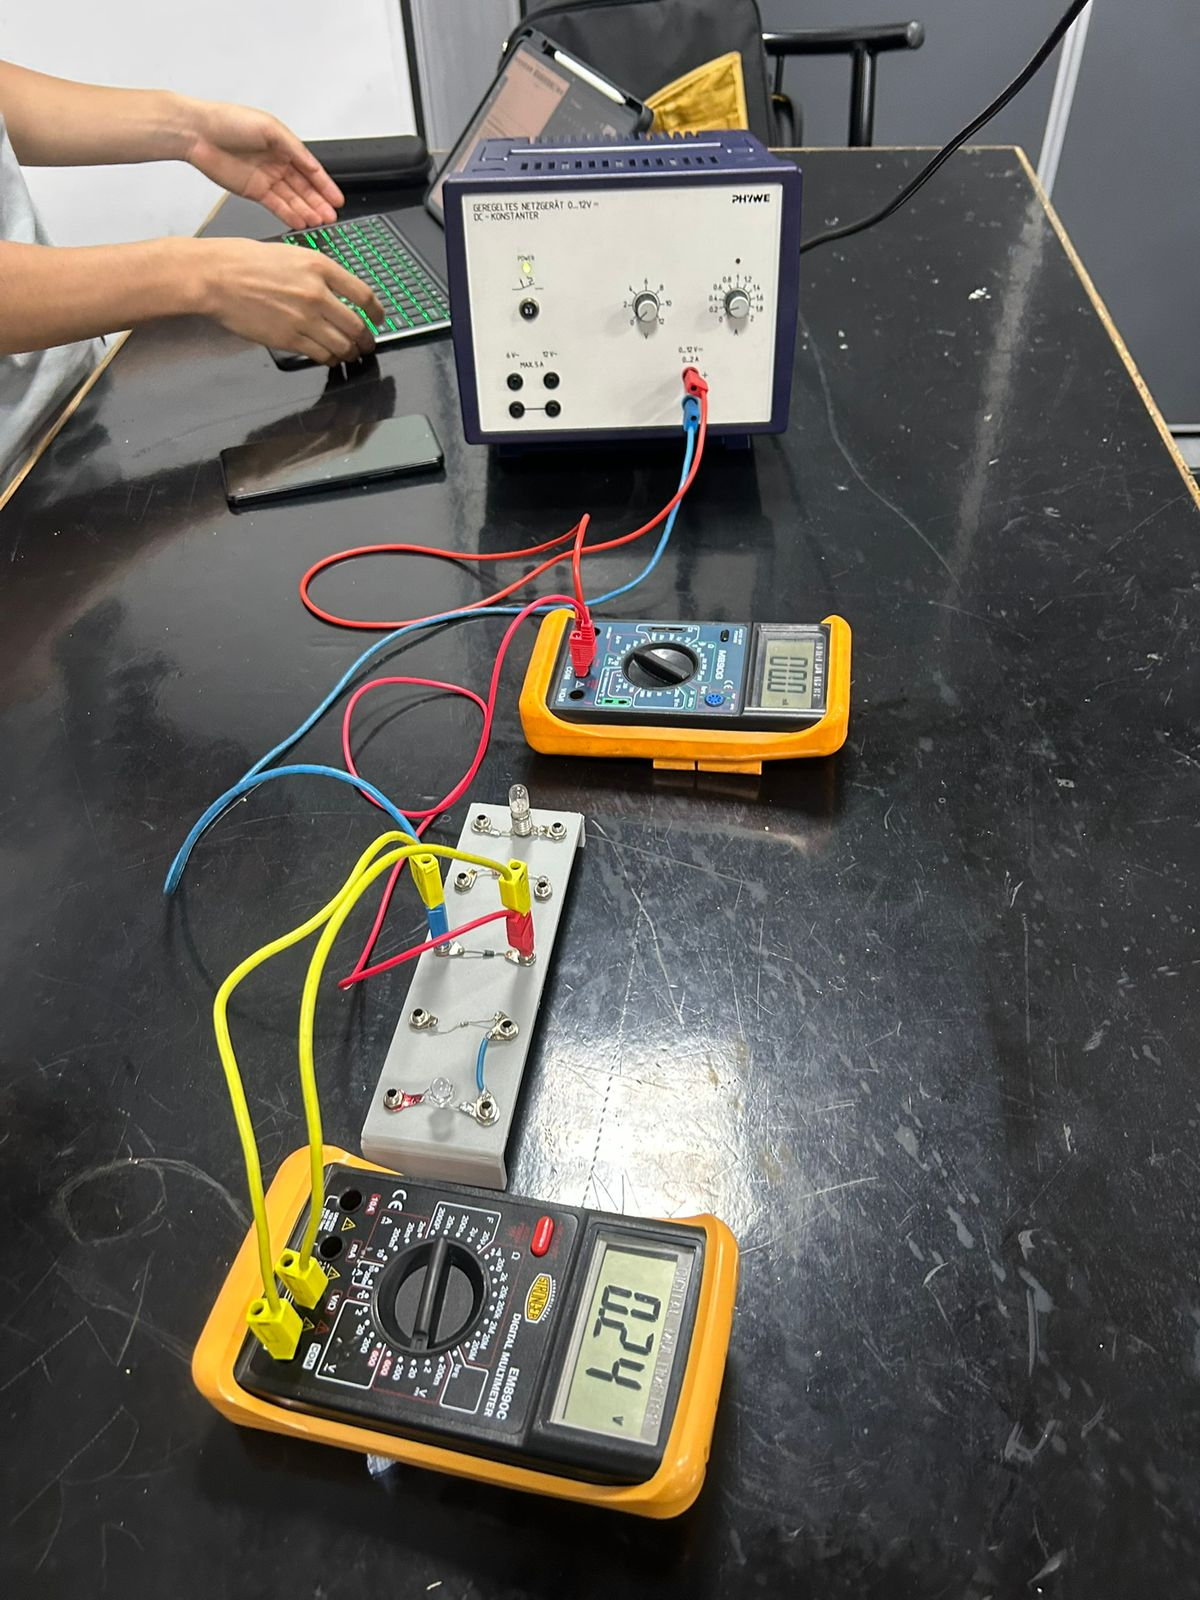
\includegraphics[width=0.8\textwidth]{foto_elementos.jpeg} 
    \caption{Disposición de los instrumentos de medición y componentes en el banco de trabajo, junto con la fuente de tensión.}
    \label{fig:fotos_laboratorio}
\end{figure}

\vspace{0.4cm}

\subsection{Circuitos de medición}
El montaje experimental se realizó siguiendo los esquemas de la Figura \ref{fig:circuitos_detallados}. Se optó por una configuración de medición donde el voltímetro mide directamente la tensión sobre el componente, asegurando que la resistencia interna del instrumento no afectara significativamente los resultados dada la magnitud de las corrientes medidas.

\vspace{0.3cm}

\begin{figure}[H]
    \centering
    % --- SUBFIGURA 1: RESISTOR ---
    \begin{subfigure}{0.48\textwidth}
        \centering
        \begin{circuitikz}[scale=0.8, transform shape]
            \draw (0,0) to[american voltage source, invert, l=$V_{f}$] (0,3)
            to[ammeter, l=$I$] (3,3)
            to[R, l=$R$, *-, v=$V_R$] (3,0)
            (3,3) -- (5,3)
            to[voltmeter, l=$V$] (5,0) -- (0,0);
        \end{circuitikz}
        \caption{Resistor de carbón ($\SI{220}{\ohm}$)}
        \label{fig:circ_resistor}
    \end{subfigure}
    \hfill
    % --- SUBFIGURA 2: LÁMPARA ---
    \begin{subfigure}{0.48\textwidth}
        \centering
        \begin{circuitikz}[scale=0.8, transform shape]
            \draw (0,0) to[american voltage source, invert, l=$V_{f}$] (0,3)
            to[ammeter, l=$I$] (3,3)
            to[lamp, l=L, *-, v=$V_L$] (3,0)
            (3,3) -- (5,3)
            to[voltmeter, l=$V$] (5,0) -- (0,0);
        \end{circuitikz}
        \caption{Lámpara de filamento}
        \label{fig:circ_lampara}
    \end{subfigure}

    \vspace{0.8cm}

    % --- SUBFIGURA 3: DIODO SILICIO ---
    \begin{subfigure}{0.48\textwidth}
        \centering
        \begin{circuitikz}[scale=0.8, transform shape]
            \draw (0,0) to[american voltage source, invert, l=$V_{f}$] (0,3)
            to[ammeter, l=$I$] (3,3)
            to[D, l=D, *-, v=$V_D$] (3,0)
            (3,3) -- (5,3)
            to[voltmeter, l=$V$] (5,0) -- (0,0);
        \end{circuitikz}
        \caption{Diodo de Silicio}
        \label{fig:circ_diodo}
    \end{subfigure}
    \hfill
    % --- SUBFIGURA 4: LED CON RESISTENCIA (Voltímetro solo en LED) ---
    \begin{subfigure}{0.48\textwidth}
        \centering
        \begin{circuitikz}[scale=0.8, transform shape]
            \draw (0,0) to[american voltage source, invert, l=$V_{f}$] (0,3)
            to[ammeter, l=$I$] (3,3)
            to[R, l=$R_p$] (3,1.5)                % Resistencia de protección hasta el punto medio
            to[led, l=LED, *-, v=$V_{LED}$] (3,0)
            
            % Conexión del voltímetro desde el nodo intermedio (3, 1.5)
            (3,1.5) -- (5,1.5) 
            to[voltmeter, l=$V$] (5,0) -- (0,0);
        \end{circuitikz}
        \caption{LED con resistencia de protección}
        \label{fig:circ_led}
    \end{subfigure}

    \caption{Esquemas eléctricos para el relevamiento de cada componente.}
    \label{fig:circuitos_detallados}
\end{figure}

\pagebreak

\pagebreak
% 6. Llamada a la sección de datos obtenidos
\section{Datos obtenidos: discusión y cálculo de errores}

A continuación se presentan los datos relevados para cada componente y sus respectivas curvas características $I=f(V)$. 

\subsection{Resistor de Carbón Depositado}

El resistor ensayado tenía un valor nominal de $R_{nom} = \SI{220}{\ohm}$ con una tolerancia del 5\% (asumida por el código de colores). Al medirlo con el multímetro, se obtuvo un valor estático de $R_{med} = \SI{216}{\ohm}$.

Luego, los datos experimentales de tensión y corriente se tabularon (Tabla \ref{tab:res_220} del Anexo) y graficaron, mostrando un comportamiento lineal típico de un dispositivo óhmico (Figura \ref{fig:curva_resistor}).


\begin{figure}[H]
    \centering
    \begin{tikzpicture}
        \begin{axis}[
            width=10cm, height=6cm,
            xlabel={Tensión (V)}, ylabel={Corriente (mA)},
            grid=major,
            legend pos=north west
        ]
        \addplot[color=blue, mark=*] coordinates {
            (0.03,0) (1.14,5.2) (2.0,9.2) (3.1,14.2) (3.84,17.6) 
            (4.85,22.3) (6.15,28.4) (6.85,31.6) (8.35,38.4) (9.09,41.8) 
            (10.23,47.1) (10.79,49.7) (12.25,56.3)
        };
        \end{axis}
    \end{tikzpicture}
    \caption{Curva característica del resistor de carbón.}
    \label{fig:curva_resistor}
\end{figure}

\textbf{Cálculo de error:}
Calculando la resistencia dinámica (pendiente de la recta) tomando los puntos extremos, se obtuvo $R_{din} = \frac{\Delta V}{\Delta I} = \frac{12.25\text{ V} - 0.03\text{ V}}{56.3\text{ mA} - 0\text{ mA}} \approx \SI{217.05}{\ohm}$. 
El error relativo porcentual respecto al valor medido con el multímetro ($\SI{216}{\ohm}$) fue:
\begin{equation}
    e\% = \left| \frac{216 - 217.05}{216} \right| \cdot 100 \approx 0.49\%
\end{equation}
Esto demuestra una excelente concordancia y confirma el comportamiento lineal.

\vspace{0.5cm}

\subsection{Lámpara de Filamento de Tungsteno}

En la Tabla \ref{tab:lampara} del Anexo se presentan los valores obtenidos durante el aumento de la tensión aplicada a la lámpara. El resultado gráfico se presenta en la Figura \ref{fig:curva_lampara} para mostrar la evolución completa de la curva característica.

\begin{figure}[H]
    \centering
    \begin{tikzpicture}
        \begin{axis}[
            width=10cm, height=6cm,
            xlabel={Tensión (V)}, ylabel={Corriente (mA)},
            grid=major, smooth
        ]
        \addplot[color=orange, mark=square*, mark size=1pt] coordinates {
            (0.02, 1.4) (0.14, 8.8) (0.35, 19.7) (0.53, 30.7) (0.72, 34.5)
            (0.97, 37.9) (1.21, 41.0) (1.38, 43.3) (1.63, 46.6) (1.92, 50.8)
            (2.10, 53.2) (2.51, 58.2) (2.90, 62.9) (3.32, 67.8) (3.92, 74.3)
            (4.53, 80.5) (4.81, 83.3) (5.24, 87.4) (5.82, 92.3) (6.18, 95.6)
            (6.41, 97.6) (6.71, 100.2) (6.87, 101.3) (7.28, 104.6) (7.73, 108.0)
            (7.87, 109.1) (8.09, 111.4) (8.56, 114.1) (8.99, 117.4) (9.75, 121.7)
            (10.26, 124.1) (10.72, 128.0) (11.16, 131.5) (12.14, 138.8)
        };
        \end{axis}
    \end{tikzpicture}
    \caption{Curva característica de la lámpara de tungsteno.}
    \label{fig:curva_lampara}
\end{figure}

\textbf{Análisis de la Resistencia Térmica en la Lámpara}: 
Por otro lado, para cada valor de V e I se calculó la resistencia estática asociada $R = V/I$ para comprobar el Efecto Joule. Los resultados se presentan en la Figura \ref{fig:curva_resistencia_lampara} a continuación.

\begin{figure}[H]
    \centering
    \begin{tikzpicture}
        \begin{axis}[
            width=10cm, height=6cm,
            xlabel={Tensión (V)}, ylabel={Resistencia ($\Omega$)},
            grid=major, smooth,
            xmin=0, xmax=13,
            ymin=0, ymax=100
        ]
        \addplot[color=orange, mark=square*, mark size=1pt] coordinates {
            (0.02,14.29) (0.14,15.91) (0.35,17.77) (0.53,17.26) (0.72,20.87) 
            (0.97,25.59) (1.21,29.51) (1.38,31.87) (1.63,34.98) (1.92,37.80) 
            (2.1,39.47) (2.51,43.13) (2.9,46.10) (3.32,48.97) (3.92,52.76) 
            (4.53,56.27) (4.81,57.74) (5.24,59.95) (5.82,63.06) (6.18,64.64) 
            (6.41,65.68) (6.71,66.97) (6.87,67.82) (7.28,69.60) (7.73,71.57) 
            (7.87,72.14) (8.09,72.62) (8.56,75.02) (8.99,76.58) (9.75,80.12) 
            (10.26,82.68) (10.72,83.75) (11.16,84.87) (12.14,87.46)
        };
        \end{axis}
    \end{tikzpicture}
    \caption{Variación de la resistencia asociada del filamento en función de la tensión aplicada.}
    \label{fig:curva_resistencia_lampara}
\end{figure}

\vspace{0.5cm}

\subsection{Diodos (Silicio y LED)}

Para los componentes semiconductores, se tabularon los valores que evidencian la tensión de umbral donde comienza la conducción abrupta (Tablas \ref{tab:led_res} y \ref{tab:diodo} del Anexo). Se presentan ambas mediciones completas gráficamente para su posterior comparación (Figuras \ref{fig:curva_diodo} y \ref{fig:curva_led}). 

\begin{figure}[H]
    \centering
    \begin{tikzpicture}
        \begin{axis}[
            width=10cm, height=6cm,
            xlabel={Tensión (V)}, ylabel={Corriente (mA)},
            grid=major,
            legend pos=north east,
            xmin=0, xmax=2.5,
            ymin=0, ymax=250
        ]
        % Diodo Silicio
        \addplot[color=black, mark=triangle*, mark size=2pt] coordinates {
            (0.0,0.0) (0.24,0.0) (0.49,0.0) (0.63,4.3) (0.737,47.0) 
            (0.753,67.5) (0.769,99.4) (0.772,108.3) (0.779,125.9) 
            (0.782,136.8) (0.791,169.4) (0.792,174) (0.797,197)
        };
        \end{axis}
    \end{tikzpicture}
    \caption{Curva característica del diodo de silicio.}
    \label{fig:curva_diodo}
\end{figure}

\begin{figure}[H]
    \centering
    \begin{tikzpicture}
        \begin{axis}[
            width=10cm, height=6cm,
            xlabel={Tensión (V)}, ylabel={Corriente (mA)},
            grid=major,
            legend pos=north east,
            xmin=0, xmax=3,
            ymin=0, ymax=20
        ]        
        % LED Rojo
        \addplot[color=red, mark=diamond*, mark size=2pt] coordinates {
            (0,0) (0.2,0) (0.27,0) (0.46,0) (0.68,0) 
            (1.12,0) (1.32,0) (1.6,0) (1.86,0) (2.13,0) 
            (2.42,0.035) (2.47,0.186) (2.51,0.625) (2.53,0.924) (2.55,1.399) 
            (2.57,1.952) (2.59,2.7) (2.61,3.69) (2.63,4.45) (2.65,5.53) 
            (2.67,6.83) (2.69,8) (2.72,10.45) (2.74,12) (2.77,13.75) 
            (2.8,17.03)
        };
        \end{axis}
    \end{tikzpicture}
    \caption{Curva característica del LED rojo.}
    \label{fig:curva_led}
\end{figure}

\textbf{Análisis Logarítmico del Diodo (Ecuación de Shockley)}: 
Para verificar el comportamiento exponencial predicho por la ecuación ideal del diodo (Ecuacion \ref{eq:shockley}), se procedió a linealizar la curva aplicando el logaritmo a la corriente medida.

Los valores nulos de corriente fueron descartados del análisis, graficando únicamente los puntos pertenecientes a la zona de conducción directa. Se puede apreciar el resultado en las siguientes figuras (\ref{fig:log_diodo_si} y \ref{fig:log_led_rojo}), donde se observa un comportamiento lineal para ambos dispositivos.

\begin{figure}[htbp]
    \centering
    \begin{tikzpicture}
        \begin{semilogyaxis}[
            width=15cm, height=10cm,
            xlabel={Tensión $V_F$ (V)},
            ylabel={Corriente $I_F$ (mA)},
            grid=both,
            minor grid style={dotted, gray!50},
            major grid style={gray!80},
            xmin=0.6, xmax=0.85, % Zoom en la zona de conducción del Si
            ymin=1, ymax=1000,
            log ticks with fixed point,
            ytick={1, 10, 100, 1000},
        ]
        \addplot[color=black, mark=triangle*, mark size=2pt] coordinates {
            (0.63,4.3) (0.737,47.0) 
            (0.753,67.5) (0.769,99.4) (0.772,108.3) (0.779,125.9) 
            (0.782,136.8) (0.791,169.4) (0.792,174) (0.797,197)
        };
        \end{semilogyaxis}
    \end{tikzpicture}
    \caption{Curva característica semilogarítmica de tensión-corriente para un diodo de silicio en polarización directa.}
    \label{fig:log_diodo_si}
\end{figure}

\begin{figure}[htbp]
    \centering
    \begin{tikzpicture}
        \begin{semilogyaxis}[
            width=15cm, height=10cm,
            xlabel={Tensión $V_F$ (V)},
            ylabel={Corriente $I_F$ (mA)},
            grid=both,
            minor grid style={dotted, gray!50},
            major grid style={gray!80},
            xmin=2.4, xmax=2.85,
            ymin=0.01, ymax=100,
            log ticks with fixed point,
            ytick={0.01, 0.1, 1, 10, 100},
        ]
        \addplot[color=red, mark=diamond*, mark size=2pt] coordinates {            
            (2.42,0.035) (2.47,0.186) (2.51,0.625) (2.53,0.924) (2.55,1.399) 
            (2.57,1.952) (2.59,2.7) (2.61,3.69) (2.63,4.45) (2.65,5.53) 
            (2.67,6.83) (2.69,8) (2.72,10.45) (2.74,12) (2.77,13.75) 
            (2.8,17.03)
        };
        \end{semilogyaxis}
    \end{tikzpicture}
    \caption{Curva característica semilogarítmica de tensión-corriente para un diodo LED rojo en polarización directa.}
    \label{fig:log_led_rojo}
\end{figure}

\pagebreak
% 7. Llamada a la sección de análisis de resultados
\section{Análisis de los resultados obtenidos}

El relevamiento de las curvas características permitió corroborar experimentalmente los modelos teóricos propuestos para los diferentes tipos de componentes.

\subsection{Componente Lineal (Resistor)}
A partir del Gráfico \ref{fig:curva_resistor}, se observa que los datos empíricos del resistor de carbón se ajustan perfectamente a una línea recta que pasa por el origen. Esto confirma su carácter de dispositivo óhmico. El mínimo margen de error (aproximadamente $0.5\%$) entre el valor estático leído por el multímetro y el valor dinámico obtenido de la pendiente demuestra que la resistencia se mantuvo constante frente a las variaciones de tensión y corriente, sin manifestar efectos de calentamiento que alteren su comportamiento.

\subsection{Componente No Lineal Térmico (Lámpara)}
El comportamiento de la lámpara de filamento (Gráfico \ref{fig:curva_lampara}) difiere radicalmente del resistor. Si bien la curva parte del origen, su pendiente disminuye a medida que aumenta la tensión. Al calcular la resistencia aparente punto a punto (Grafico \ref{fig:curva_resistencia_lampara}), se evidencia un marcado aumento: a tensiones muy bajas ($0.02$ V) la resistencia es de aproximadamente $\SI{14}{\ohm}$, mientras que a $12.14$ V asciende a más de $\SI{87}{\ohm}$. 

Este fenómeno es la comprobación práctica del efecto Joule y del coeficiente de temperatura positivo (PTC) del tungsteno. Al aumentar la tensión, aumenta la corriente, lo que eleva significativamente la temperatura del filamento (haciéndolo brillar) y, en consecuencia, aumenta su resistividad, ofreciendo mayor oposición al paso de corriente.

\subsection{Componentes de Estado Sólido (Diodos)}
Las curvas del diodo de silicio y del LED (Gráficos \ref{fig:curva_diodo} y \ref{fig:curva_led}) corroboran la fuerte no linealidad y asimetría de los componentes semiconductores.

En ambos casos, la corriente es prácticamente nula hasta alcanzar una tensión de umbral específica para cada material, a partir de la cual la curva adopta un perfil casi exponencial. Al graficar la curva característica semilogarítmica de tensión-corriente (Figuras \ref{fig:log_diodo_si} y \ref{fig:log_led_rojo}), se observa claramente una tendencia lineal (una recta) para ambos componentes en su respectiva zona de polarización directa. Esto corrobora empíricamente que el modelo matemático exponencial describe de forma precisa la física de ambos dispositivos. 

Asimismo, la separación horizontal entre ambas rectas evidencia la gran diferencia en la barrera de potencial (tensión de umbral) que existe entre el silicio estándar y el material compuesto utilizado para el LED rojo:
\begin{itemize}
    \item Para el \textbf{Diodo de Silicio}, se observa que comienza a conducir de manera notoria superando la barrera de los $0.6$ V - $0.7$ V, de acuerdo con la teoría clásica de uniones P-N de silicio.
    \item Para el \textbf{LED Rojo}, el codo de la curva se encuentra desplazado, comenzando la conducción alrededor de los $2.4$ V - $2.5$ V. Esto responde al salto energético mayor requerido por los semiconductores compuestos utilizados para emitir fotones en el espectro visible rojo. 
\end{itemize}

Cabe destacar que la abrupta pendiente de ambos componentes una vez superada su tensión de umbral ratifica la necesidad práctica de utilizar resistencias limitadoras (como la empleada de $\SI{560}{\ohm}$), ya que un pequeño incremento en la tensión de la fuente se traduce en un aumento drástico y potencialmente destructivo de la corriente.

\pagebreak
% 8. Llamada a la sección de anexo
\section{Anexo: Tablas de mediciones detalladas}

% Tabla 1: Resistencia 220 ohm
\begin{table}[htpb]
    \centering
    \begin{tabular}{cc}
        \toprule
        Corriente $I$ (mA) & Tensión $V_R$ (V) \\
        \midrule
        0	& 0.03 \\
        5.2	& 1.14 \\
        9.2	& 2.00 \\
        14.2	& 3.1 \\
        17.6	& 3.84 \\
        22.3	& 4.85 \\
        28.4	& 6.15 \\
        31.6	& 6.85 \\
        38.4	& 8.35 \\
        41.8	& 9.09 \\
        47.1	& 10.23 \\
        49.7	& 10.79 \\
        56.3	& 12.25 \\
        \bottomrule
    \end{tabular}
    \caption{Mediciones para la Resistencia de 220 $\Omega$.}
    \label{tab:res_220}
\end{table}

% Tabla 2: Lámpara
\begin{table}[htpb]
    \centering
    \begin{tabular}{ccc}
        \toprule
        Corriente $I$ (mA) & Tensión $V_L$ (V) \\
        \midrule
        1.4 &	0.02 \\
        8.8 &	0.14 \\
        19.7 &	0.35 \\
        30.7 &	0.53 \\
        34.5 &	0.72 \\
        37.9 &	0.97 \\
        41 &	1.21 \\
        43.3 &	1.38 \\
        46.6 &	1.63 \\
        50.8 &	1.92 \\
        53.2 &	2.1 \\
        58.2 &	2.51 \\
        62.9 &	2.9 \\
        67.8 &	3.32 \\
        74.3 &	3.92 \\
        80.5 &	4.53 \\
        83.3 &	4.81 \\
        87.4 &	5.24 \\
        92.3 &	5.82 \\
        95.6 &	6.18 \\
        97.6 &	6.41 \\
        100.2 &	6.71 \\
        101.3 &	6.87 \\
        104.6 &	7.28 \\
        108 &	7.73 \\
        109.1 &	7.87 \\
        111.4 &	8.09 \\
        114.1 &	8.56 \\
        117.4 &	8.99 \\
        121.7 &	9.75 \\
        124.1 &	10.26 \\
        128 &	10.72 \\
        131.5 &	11.16 \\
        138.8 &	12.14 \\
        \bottomrule
    \end{tabular}
    \caption{Mediciones para la Lámpara incandescente.}
    \label{tab:lampara}
\end{table}

% Tabla 3: LED + Resistencia
\begin{table}[htpb]
    \centering
    \begin{tabular}{ccc}
        \toprule
        Corriente $I$ (mA) & Tensión $V_{LED}$ (V)\\
        \midrule
        0 & 0 \\
        0 & 0.2 \\
        0 & 0.27 \\
        0 & 0.46 \\
        0 & 0.68 \\
        0 & 1.12 \\
        0 & 1.32 \\
        0 & 1.6 \\
        0 & 1.86 \\
        0 & 2.13 \\
        0.035 & 2.42 \\
        0.186 & 2.47 \\
        0.625 & 2.51 \\
        0.924 & 2.53 \\
        1.399 & 2.55 \\
        1.952 & 2.57 \\
        2.7	& 2.59 \\
        3.69 & 2.61 \\
        4.45 & 2.63 \\
        5.53  & 2.65 \\
        6.83 & 2.67 \\
        8 & 2.69 \\
        10.45 & 2.72 \\
        12 & 2.74 \\
        13.75 & 2.77 \\
        17.03 & 2.8 \\
        \bottomrule
    \end{tabular}
    \caption{Mediciones para el LED en serie con resistencia de 560 $\Omega$.}
    \label{tab:led_res}
\end{table}

% Tabla 4: Diodo
\begin{table}[htpb]
    \centering
    \begin{tabular}{ccc}
        \toprule
        Corriente $I$ (mA) & Tensión $V_D$ (V) \\
        \midrule
        0 &	0 \\
        0	& 0.24 \\
        0	& 0.49 \\
        4.3	& 0.63 \\
        47	& 0.737 \\
        67.5	& 0.753 \\
        99.4	& 0.769 \\
        108.3	& 0.772 \\
        125.9	& 0.779 \\
        136.8	& 0.782 \\
        169.4	& 0.791 \\
        174	& 0.792 \\
        197	& 0.797 \\
        \bottomrule
    \end{tabular}
    \caption{Mediciones para el Diodo.}
    \label{tab:diodo}
\end{table}

\end{document}
